% Options for packages loaded elsewhere
\PassOptionsToPackage{unicode}{hyperref}
\PassOptionsToPackage{hyphens}{url}
%
\documentclass[
]{article}
\usepackage{amsmath,amssymb}
\usepackage{iftex}
\ifPDFTeX
  \usepackage[T1]{fontenc}
  \usepackage[utf8]{inputenc}
  \usepackage{textcomp} % provide euro and other symbols
\else % if luatex or xetex
  \usepackage{unicode-math} % this also loads fontspec
  \defaultfontfeatures{Scale=MatchLowercase}
  \defaultfontfeatures[\rmfamily]{Ligatures=TeX,Scale=1}
\fi
\usepackage{lmodern}
\ifPDFTeX\else
  % xetex/luatex font selection
\fi
% Use upquote if available, for straight quotes in verbatim environments
\IfFileExists{upquote.sty}{\usepackage{upquote}}{}
\IfFileExists{microtype.sty}{% use microtype if available
  \usepackage[]{microtype}
  \UseMicrotypeSet[protrusion]{basicmath} % disable protrusion for tt fonts
}{}
\makeatletter
\@ifundefined{KOMAClassName}{% if non-KOMA class
  \IfFileExists{parskip.sty}{%
    \usepackage{parskip}
  }{% else
    \setlength{\parindent}{0pt}
    \setlength{\parskip}{6pt plus 2pt minus 1pt}}
}{% if KOMA class
  \KOMAoptions{parskip=half}}
\makeatother
\usepackage{xcolor}
\usepackage[margin=1in]{geometry}
\usepackage{graphicx}
\makeatletter
\newsavebox\pandoc@box
\newcommand*\pandocbounded[1]{% scales image to fit in text height/width
  \sbox\pandoc@box{#1}%
  \Gscale@div\@tempa{\textheight}{\dimexpr\ht\pandoc@box+\dp\pandoc@box\relax}%
  \Gscale@div\@tempb{\linewidth}{\wd\pandoc@box}%
  \ifdim\@tempb\p@<\@tempa\p@\let\@tempa\@tempb\fi% select the smaller of both
  \ifdim\@tempa\p@<\p@\scalebox{\@tempa}{\usebox\pandoc@box}%
  \else\usebox{\pandoc@box}%
  \fi%
}
% Set default figure placement to htbp
\def\fps@figure{htbp}
\makeatother
\setlength{\emergencystretch}{3em} % prevent overfull lines
\providecommand{\tightlist}{%
  \setlength{\itemsep}{0pt}\setlength{\parskip}{0pt}}
\setcounter{secnumdepth}{-\maxdimen} % remove section numbering
% definitions for citeproc citations
\NewDocumentCommand\citeproctext{}{}
\NewDocumentCommand\citeproc{mm}{%
  \begingroup\def\citeproctext{#2}\cite{#1}\endgroup}
\makeatletter
 % allow citations to break across lines
 \let\@cite@ofmt\@firstofone
 % avoid brackets around text for \cite:
 \def\@biblabel#1{}
 \def\@cite#1#2{{#1\if@tempswa , #2\fi}}
\makeatother
\newlength{\cslhangindent}
\setlength{\cslhangindent}{1.5em}
\newlength{\csllabelwidth}
\setlength{\csllabelwidth}{3em}
\newenvironment{CSLReferences}[2] % #1 hanging-indent, #2 entry-spacing
 {\begin{list}{}{%
  \setlength{\itemindent}{0pt}
  \setlength{\leftmargin}{0pt}
  \setlength{\parsep}{0pt}
  % turn on hanging indent if param 1 is 1
  \ifodd #1
   \setlength{\leftmargin}{\cslhangindent}
   \setlength{\itemindent}{-1\cslhangindent}
  \fi
  % set entry spacing
  \setlength{\itemsep}{#2\baselineskip}}}
 {\end{list}}
\usepackage{calc}
\newcommand{\CSLBlock}[1]{\hfill\break\parbox[t]{\linewidth}{\strut\ignorespaces#1\strut}}
\newcommand{\CSLLeftMargin}[1]{\parbox[t]{\csllabelwidth}{\strut#1\strut}}
\newcommand{\CSLRightInline}[1]{\parbox[t]{\linewidth - \csllabelwidth}{\strut#1\strut}}
\newcommand{\CSLIndent}[1]{\hspace{\cslhangindent}#1}
\usepackage{booktabs}
\usepackage{longtable}
\usepackage{array}
\usepackage{multirow}
\usepackage{wrapfig}
\usepackage{float}
\usepackage{colortbl}
\usepackage{pdflscape}
\usepackage{tabu}
\usepackage{threeparttable}
\usepackage{threeparttablex}
\usepackage[normalem]{ulem}
\usepackage{makecell}
\usepackage{xcolor}
\usepackage{bookmark}
\IfFileExists{xurl.sty}{\usepackage{xurl}}{} % add URL line breaks if available
\urlstyle{same}
\hypersetup{
  pdftitle={Assessing feature importance for sgRNA using supervised machine learning},
  pdfauthor={Alec Thomsen, Emil Carlstedt},
  hidelinks,
  pdfcreator={LaTeX via pandoc}}

\title{Assessing feature importance for sgRNA using supervised machine
learning}
\author{Alec Thomsen, Emil Carlstedt}
\date{2025-05-29}

\begin{document}
\maketitle

\subsection{Introduction}\label{introduction}

The discovery of CRISPR-Cas9 has led to innumerable possibilities in the
field of biotechnology. One of them involves the use of single-guide RNA
engineered to target specific genes of interest in order to do knock-out
experiments. Understanding how to design these sgRNAs is crucial to the
experiments success, therefore guide lines have been developed. Although
the guidelines differ for different species they have been shown to be
effective.(Schindele \emph{et al.} 2020) Our interest is to find out
just which of the features are most important for the efficiency of the
sgRNA. To tackle this issue we will employ a tactic involving supervised
machine learning. This will help us assess what features of a sgRNA are
most important for its effectiveness.

\subsection{Theory}\label{theory}

The sgRNA dataset we chose to use was of the GeCKO v2 sgRNA library, and
it was designed to give high-throughput genome wide knockout screening
Therefore when using this data we assume that these sgRNA's reliably
bind to their respective target binding site, and bind with high
accuracy.

\subsection{Implementation}\label{implementation}

\begin{enumerate}
\def\labelenumi{\arabic{enumi}.}
\tightlist
\item
  Flowchart or overview of the solution; link to GitHub\\
\item
  Relevant Screenshots of the RShiny solution\\
\item
  Bonus material - additional tasks you added that you want to share
  with the others
\end{enumerate}

\subsubsection{Pre-Processing}\label{pre-processing}

The features of interest; nucleotide position, gc content, exon
position, and RNA sequencing expression were extracted from the
database. NA values were omitted and RNA-seq expression was log2
transformed for easier interpretation. Only the sgRNA with RNA-seq
expression above 1 were kept as they interpreted as actively transcribed
genes. An initial look at the distribution of the features was done
using a box plot (See \emph{Figure 1}). This identified a skewed
distribution of the data, especially in the feature exon position.

\begin{figure}

{\centering 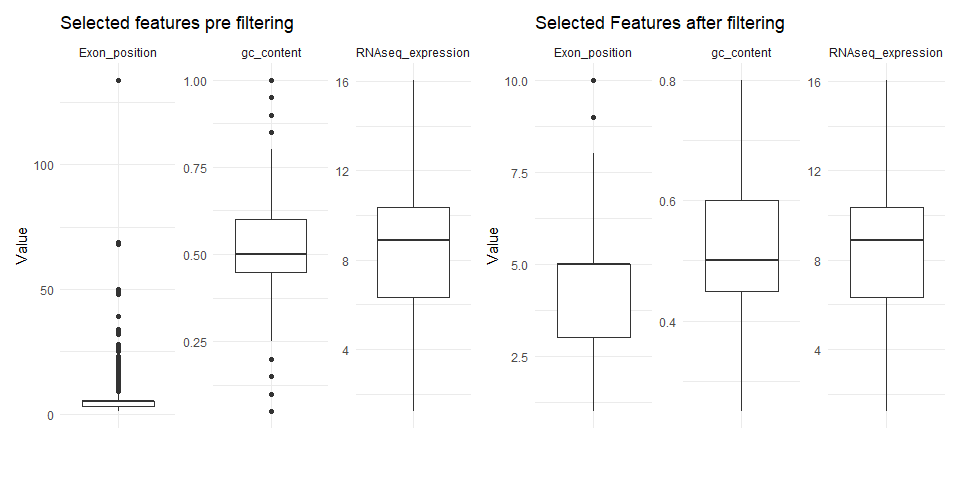
\includegraphics{report_files/figure-latex/unnamed-chunk-1-1} 

}

\caption{Figure 1. Boxplots displaying the distribution of selected features (exon_position, gc_content, and RNAseq_expression). The plot to the left displays the data pre filtering and the one on the right after filtering. Looking specifically on the boxplot for exon_position we can see that there are a outliers that skews the data, this is adress by the removal of the outliers.}\label{fig:unnamed-chunk-1}
\end{figure}

We then filtered the data, only keeping those with a negative LFC. We
then used the absolute value of the LFC as our dependent variable for
the model.\\
The data was split into training and test sets using a 80/20 split.
Using the hyper parameters seen in \emph{Table 1}, the model underwent a
5-fold cross-validation, for 1000 rounds with early stopping after 10,
in order to find the best boosting round.

\begin{longtable}[l]{>{\raggedright\arraybackslash}p{4cm}>{\raggedright\arraybackslash}p{4cm}}
\caption{\label{tab:unnamed-chunk-2}Table 1. Model Parameters}\\
\toprule
Parameter & Value\\
\midrule
eta & 0.1\\
max\_depth & 4\\
gamma & 1\\
objective & reg:squarederror\\
eval\_metric & rmse\\
\bottomrule
\end{longtable}

This resulted in a optimal boosting round of 115 which was implemented
when training the model on the training data.\\
After the training SHAP values were calculated as seen in \emph{Figure
2}. Here we can see that highly expressed genes are positively related
to a large LFC value, these genes could possible be viewed as
``householding'' genes and have a vital part in the cell. Nucleotide
position has unclear results for example position 20 where all
nucleotides have a negative impact on the model which goes against
previous studies saying that the later positions are more important.

\begin{figure}
\centering
\pandocbounded{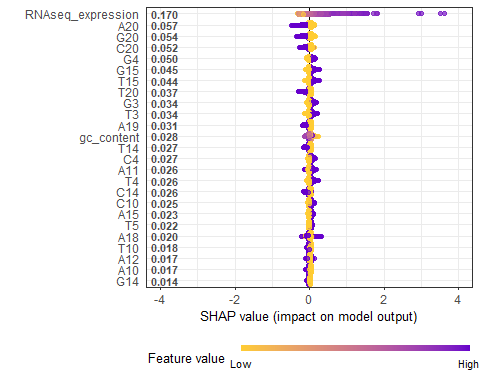
\includegraphics[keepaspectratio]{report_files/figure-latex/unnamed-chunk-3-1.pdf}}
\caption{Figure 2. SHAP values for the final model. RNA-seq expression
can be seen as the highest contributing feature to the models
prediction. Higher RNA expression leads to higher LFC.}
\end{figure}

After training the model was used to predict the LFC on the testing data
that was withheld from training. The RMSE and MAE were not that large
but the R2 was very low, meaning the model can make semi accurate
predictions but is unable to explain the variance in the data.(See
\emph{Table 2}).

\begin{longtable}[l]{>{\raggedleft\arraybackslash}p{6cm}>{\raggedleft\arraybackslash}p{4cm}r}
\caption{\label{tab:unnamed-chunk-4}Table 2. Evaluation Metrics for Final Model.}\\
\toprule
model\_rmse & model\_mae & model\_r2\\
\midrule
1.123658 & 0.7823011 & 0.1005288\\
\bottomrule
\end{longtable}

This can also be seen when looking at the Prediction vs Actual plot and
Predicted vs Residuals (See \emph{Figure 3 and 4}). The model seems
limited in its predictions to a range of 0.5 to 1.5 regardless of the
actual value of the sequence. And the fanning pattern displayed in
\emph{Figure 4} indicates heteroscadescity in the models predictions as
the error is increasing when the model tries to predict larger values.

\begin{figure}
\centering
\pandocbounded{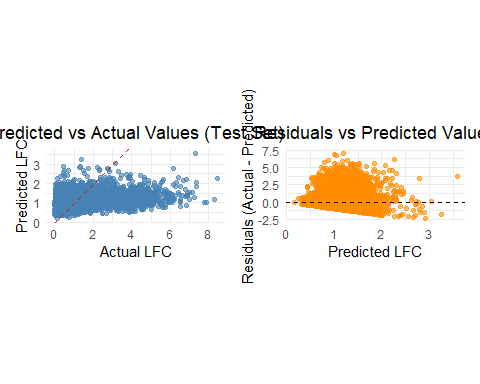
\includegraphics[keepaspectratio]{report_files/figure-latex/unnamed-chunk-5-1.pdf}}
\caption{Figure 3 (left) displaying a pattern that the model can only
predict values between 0.5 and 1.5 regardless of the actual value.
Figure 4 (right) Displaying a fanning pattern, suggesting
heteroscedascity.}
\end{figure}

\subsection{Evaluation}\label{evaluation}

Our model is unable to find a pattern in the data we trained it on and
therefore the SHAP values are not trustworthy. No conclusions towards
our original goal can be drawn based on our results.\\
This is most likely to the lack of larger scores in the data as seen in
distribution of LFC(See Figure 1A in appendix).\\
Testing different models and different targets could also be an option
for further testing if more time was available. Using LFC as a target
might not have been the best choice as we would only get on successful
knock outs that targeted a vital gene. We tried to work around this by
filtering out LFCs that were not of interest but this also means that we
loose a lot of data. Using transcriptomic data for creating a
classification on successful knock outs would result in minimum loss of
data as even non vital genes would be included. Of course there are
other difficulties with that approach. Would you use a binary approach
saying that if its below a baseline with a certain amount its regarded a
knock out or do you create different levels of success based on how much
the transcription is reduced. And how do you decide on these limits? A
lot of questions arise once you start digging into this subject and if
time allows we would like to explore them all.

\subsection{Appendix}\label{appendix}

Figure 1A

\begin{verbatim}
## `stat_bin()` using `bins = 30`. Pick better value with `binwidth`.
## `stat_bin()` using `bins = 30`. Pick better value with `binwidth`.
\end{verbatim}

\pandocbounded{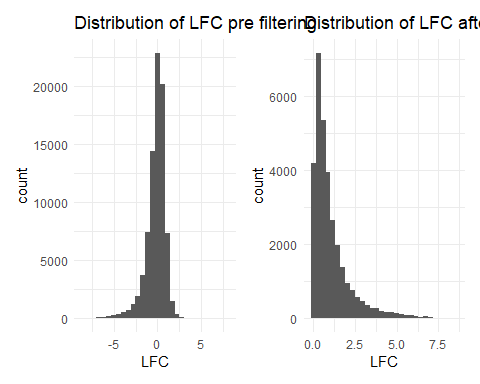
\includegraphics[keepaspectratio]{report_files/figure-latex/unnamed-chunk-6-1.pdf}}

\subsection*{References}\label{references}
\addcontentsline{toc}{subsection}{References}

\phantomsection\label{refs}
\begin{CSLReferences}{1}{0}
\bibitem[\citeproctext]{ref-schindele2020crispr}
Schindele, P., Wolter, F., and Puchta, H. (2020) {`CRISPR guide RNA
design guidelines for efficient genome editing'}, in \emph{Methods in
Molecular Biology}, Humana, New York, NY, 331--342, available:
\url{https://doi.org/10.1007/978-1-0716-0712-1_19}.

\end{CSLReferences}

\end{document}
